\section{Modellering af Semplito og dets komponenter}
\label{kabitel:ModelleringSystem}

For at sikre at vores program har så høj en kvalitet som muligt bruger vi nogle UML artefakter til at modellerer vores systems komponenter, og hvordan komponenterne skal arbejde sammen.
Dette vil blive arbejdet med i dette kapitel.

\subsection{Designklassediagram(DCD)}
\label{DCD}

For bedre at overskue associationerne mellem klasserne i vores program, samt for at give et overblik over hvilke metoder klasserne har, har vi lavet et DCD. 

DCD'et er baseret på vores objekt- og domænemodel, se afsnit \ref{objektmodel} og \ref{domaenemodel} og er blevet opdateret løbende i projektet.
DCD'et har været med til at sikre, at kodestandarden blev overholdt.
Dertil har det gjort det nemmere at bestemme ansvaret for hver klasse.

Når man laver et DCD er det vigtigt, at kravene til programmet repræsenteres, så det bliver implementeret rigtigt.
Med det menes, at en metodes signatur også skal indeholde, hvilke variabeltyper den modtager og returnerer, at metoder og variablers tilgængelighed skal kunne ses, det skal vises, hvis en klasse arver fra en anden klasse eller implementerer et interface.
Det skal også vises, hvilke klasser der kender til hinanden ved at bruge associationspile.

For at holde det overskueligt har vi både lavet et samlet DCD, men også lavet mindre DCD'er, der er bundet til en bestemt use case, og derfor kun indeholder de klasser, som er relevante for use casen.

På figur \ref{fig:DCD} kan domænelaget af DCD'en for use casen: Book Ny Aftale ses.
I bilagene på figurene \ref{bilag:RelationDCD}, \ref{bilag:UIDCD}, \ref{bilag:ApplicationDCD}, \ref{bilag:DomainDCD}, \ref{bilag:PersistableDCD} kan en samlet DCD for hele systemet ses.

% Mangler evt. noget mere om hvordan den er blevet holdt op til programmet. also pictures

\begin{sidewaysfigure}
    \caption{DCD for Semplito - Bookingsystemet}
    \centering
        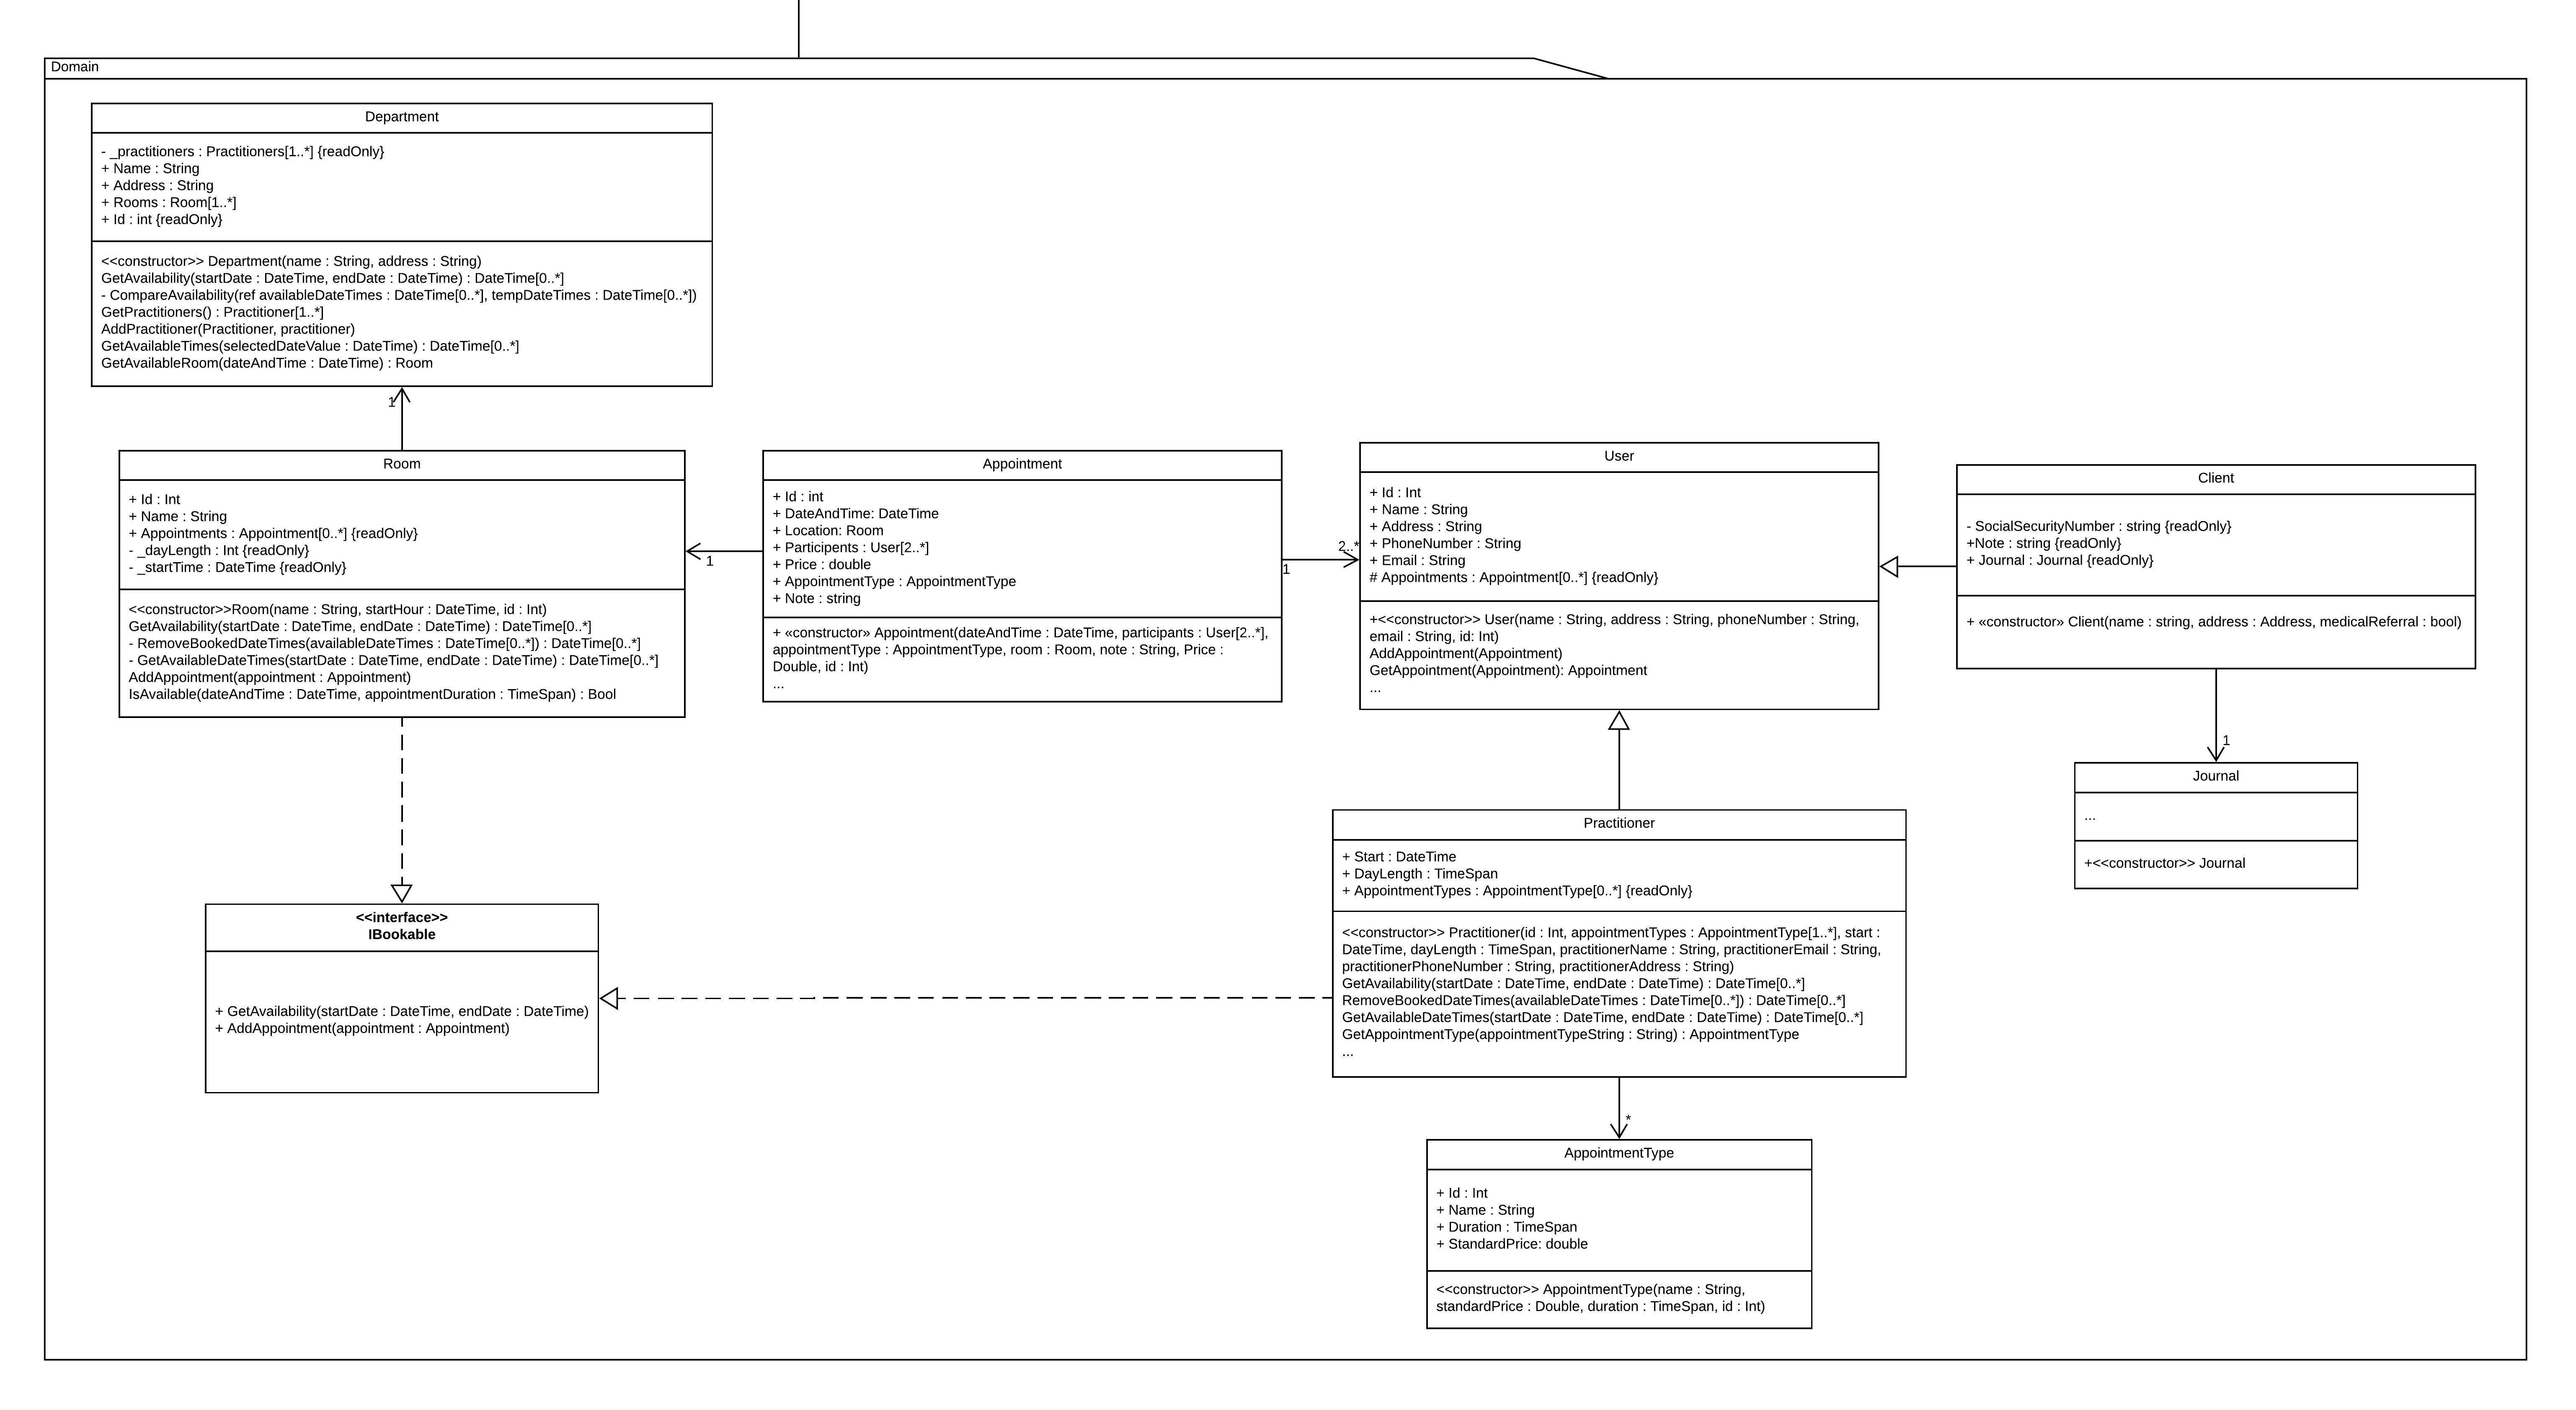
\includegraphics[width=\textwidth]{DomainDCD.png}
    \label{fig:DCD}
\end{sidewaysfigure}

\subsection{Sekvensdiagram(SD)}
\label{SD}

Et SD beskriver, hvordan softwareklasser taler sammen.
Det er vigtigt, at SD'et derfor er på samme sprog, som man ønsker ens kode skal være, da metodenavnene i SD'et er de metoder, som udvikleren implementerer.
Derfor skal metoderne også være de samme metoder som i DCD'en.

På figur \ref{fig:SD} kan et SD for SOC'en createAppointment ses.
Når en bruger trykker på 'opret aftale'-knappen i 'opret aftale'-vinduet, vil vinduet kalde controlleren, som kalder videre ned i systemet til appointmentRepo-objektet, der laver en ny aftale og tilføjer referencer til det nye appointment-objekt i det angivne room-objekt og de angivne user-objekter.
Derefter bliver der sendt en besked til de involverede brugere, hvis det er ønsket, gennem appointmentNotification-objektet, der bruger emailNotification- og smsNotificiation-objekterne.
Til sidst kalder appointmentRepo-objektet sit objekt, der implementer IPersistable-interfacet.

\begin{sidewaysfigure}
    \caption{SD for SOC Operation - createAppointment}
    \centering
        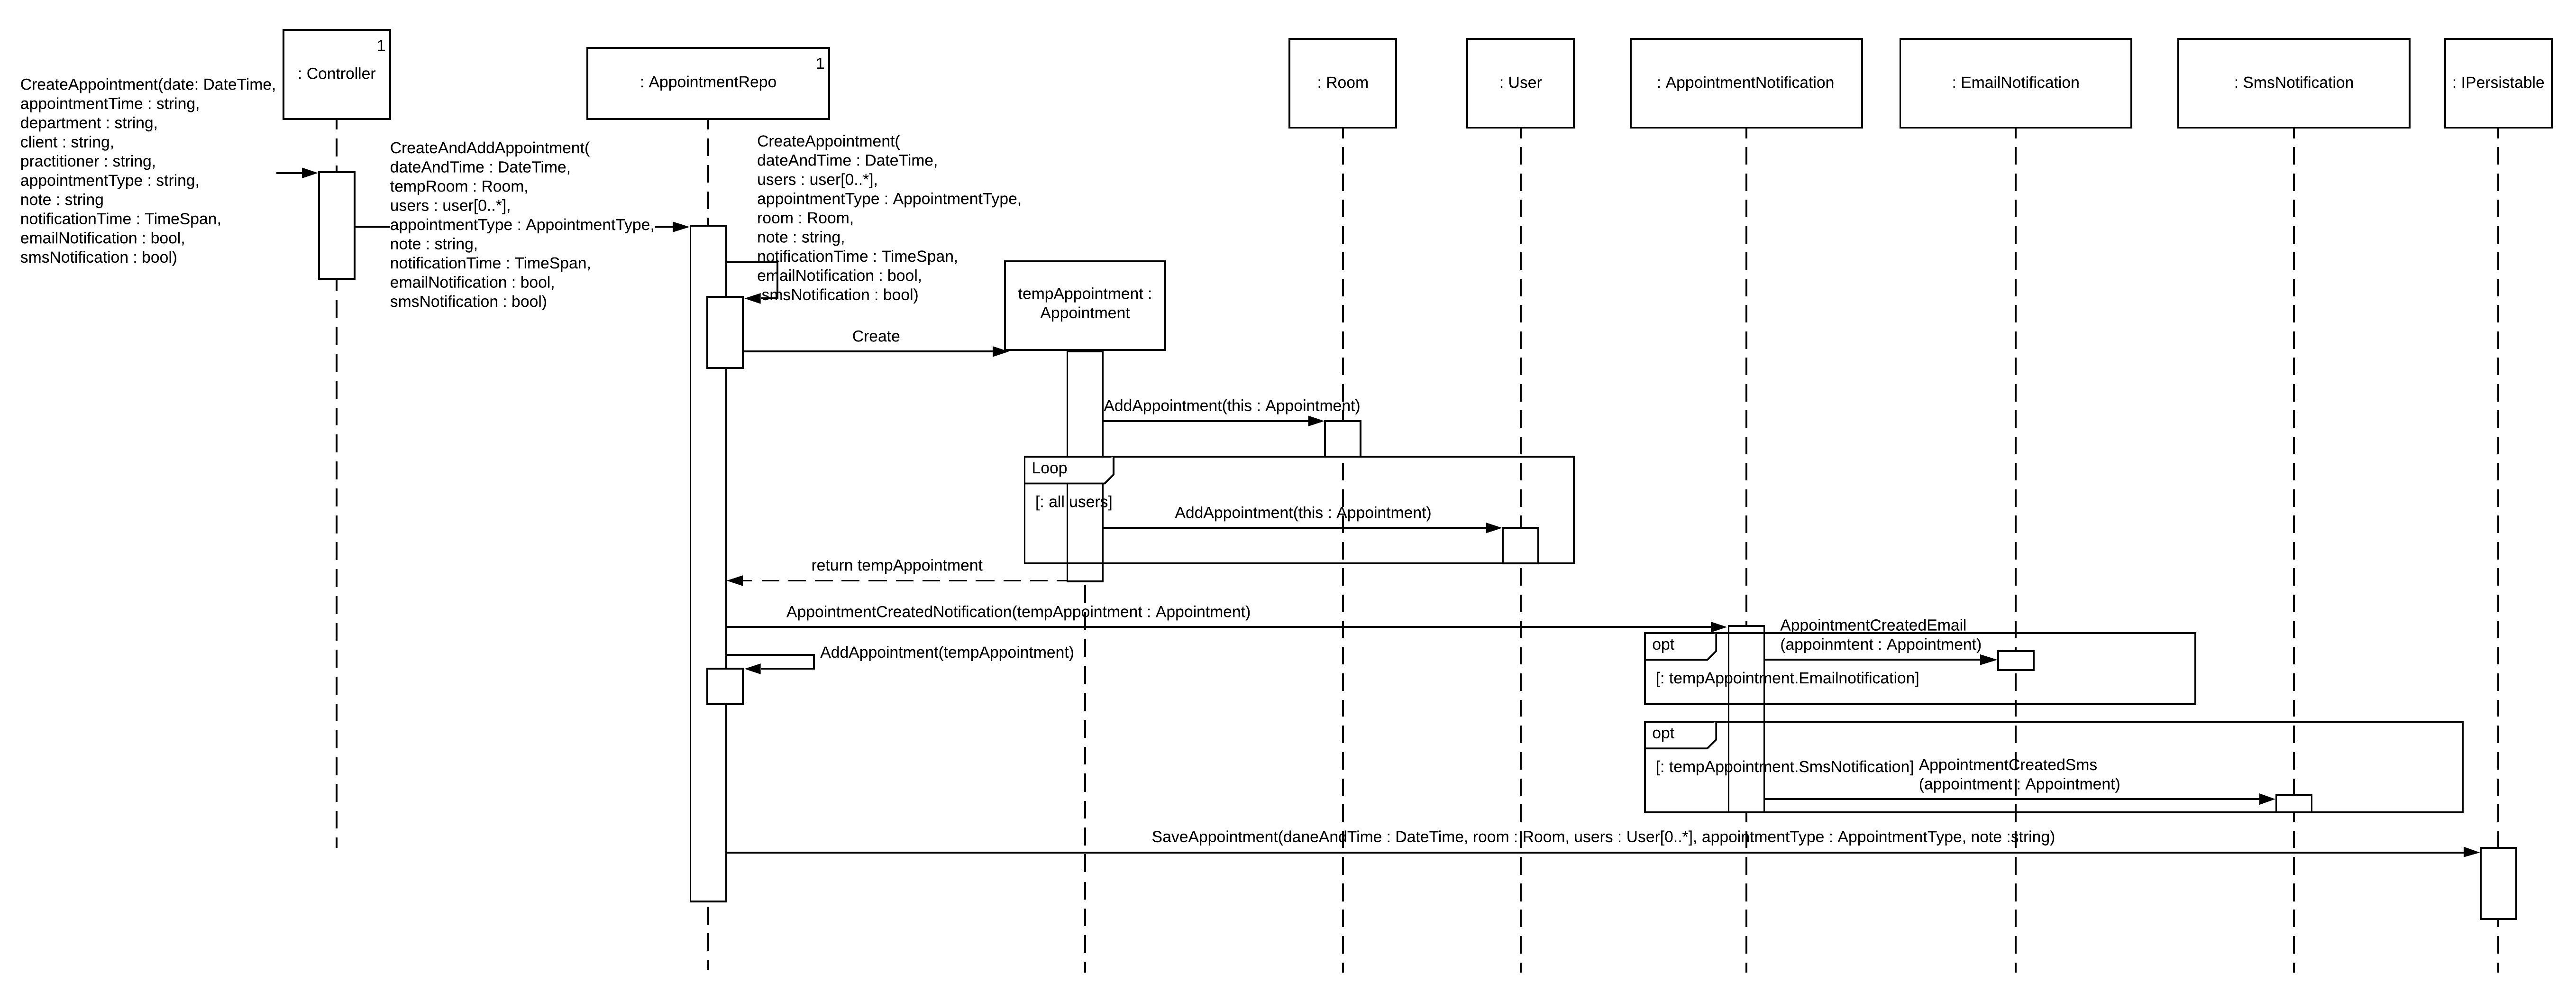
\includegraphics[width=\textwidth]{SD.png}
    \label{fig:SD}
\end{sidewaysfigure}

\subsection{Pakkediagram - Lagdeling}
\label{Pakkediagram}

Ud over vores DCD lavede vi også et pakkediagram.
Pakkediagrammet er til stor hjælp, når man skal finde rundt i programmets forskellige klasser og lag.
Ligesom DCD'et kan det give et overblik over hvilke klasser, der har kendskab til hinanden, men uden at vise metoderne, som kan gøre det sværere at overskue relationerne mellem de forskellige klasser.
Samtidigt viser pakkediagrammet mere omkring programmets lagdeling, da klasserne er opdelt i de lag, som vi har opdelt vores system i, se figur \ref{fig:pakkediagram}.

Pakkediagrammet giver os et bedre overblik over programmet som helhed, hvor DCD'et giver mulighed for at kigge nærmere på klasserne.

Både pakkediagrammet og DCD'et har været brugt i mange gode diskussioner i gruppen i forbindelse med vores valg af softwarearkitektur.
Vores valg af lagdeling vil blive diskuteret nærmere i afsnit \ref{lagdeling}.

\begin{sidewaysfigure}
    \caption{Pakkediagram for systemet}
    \centering
        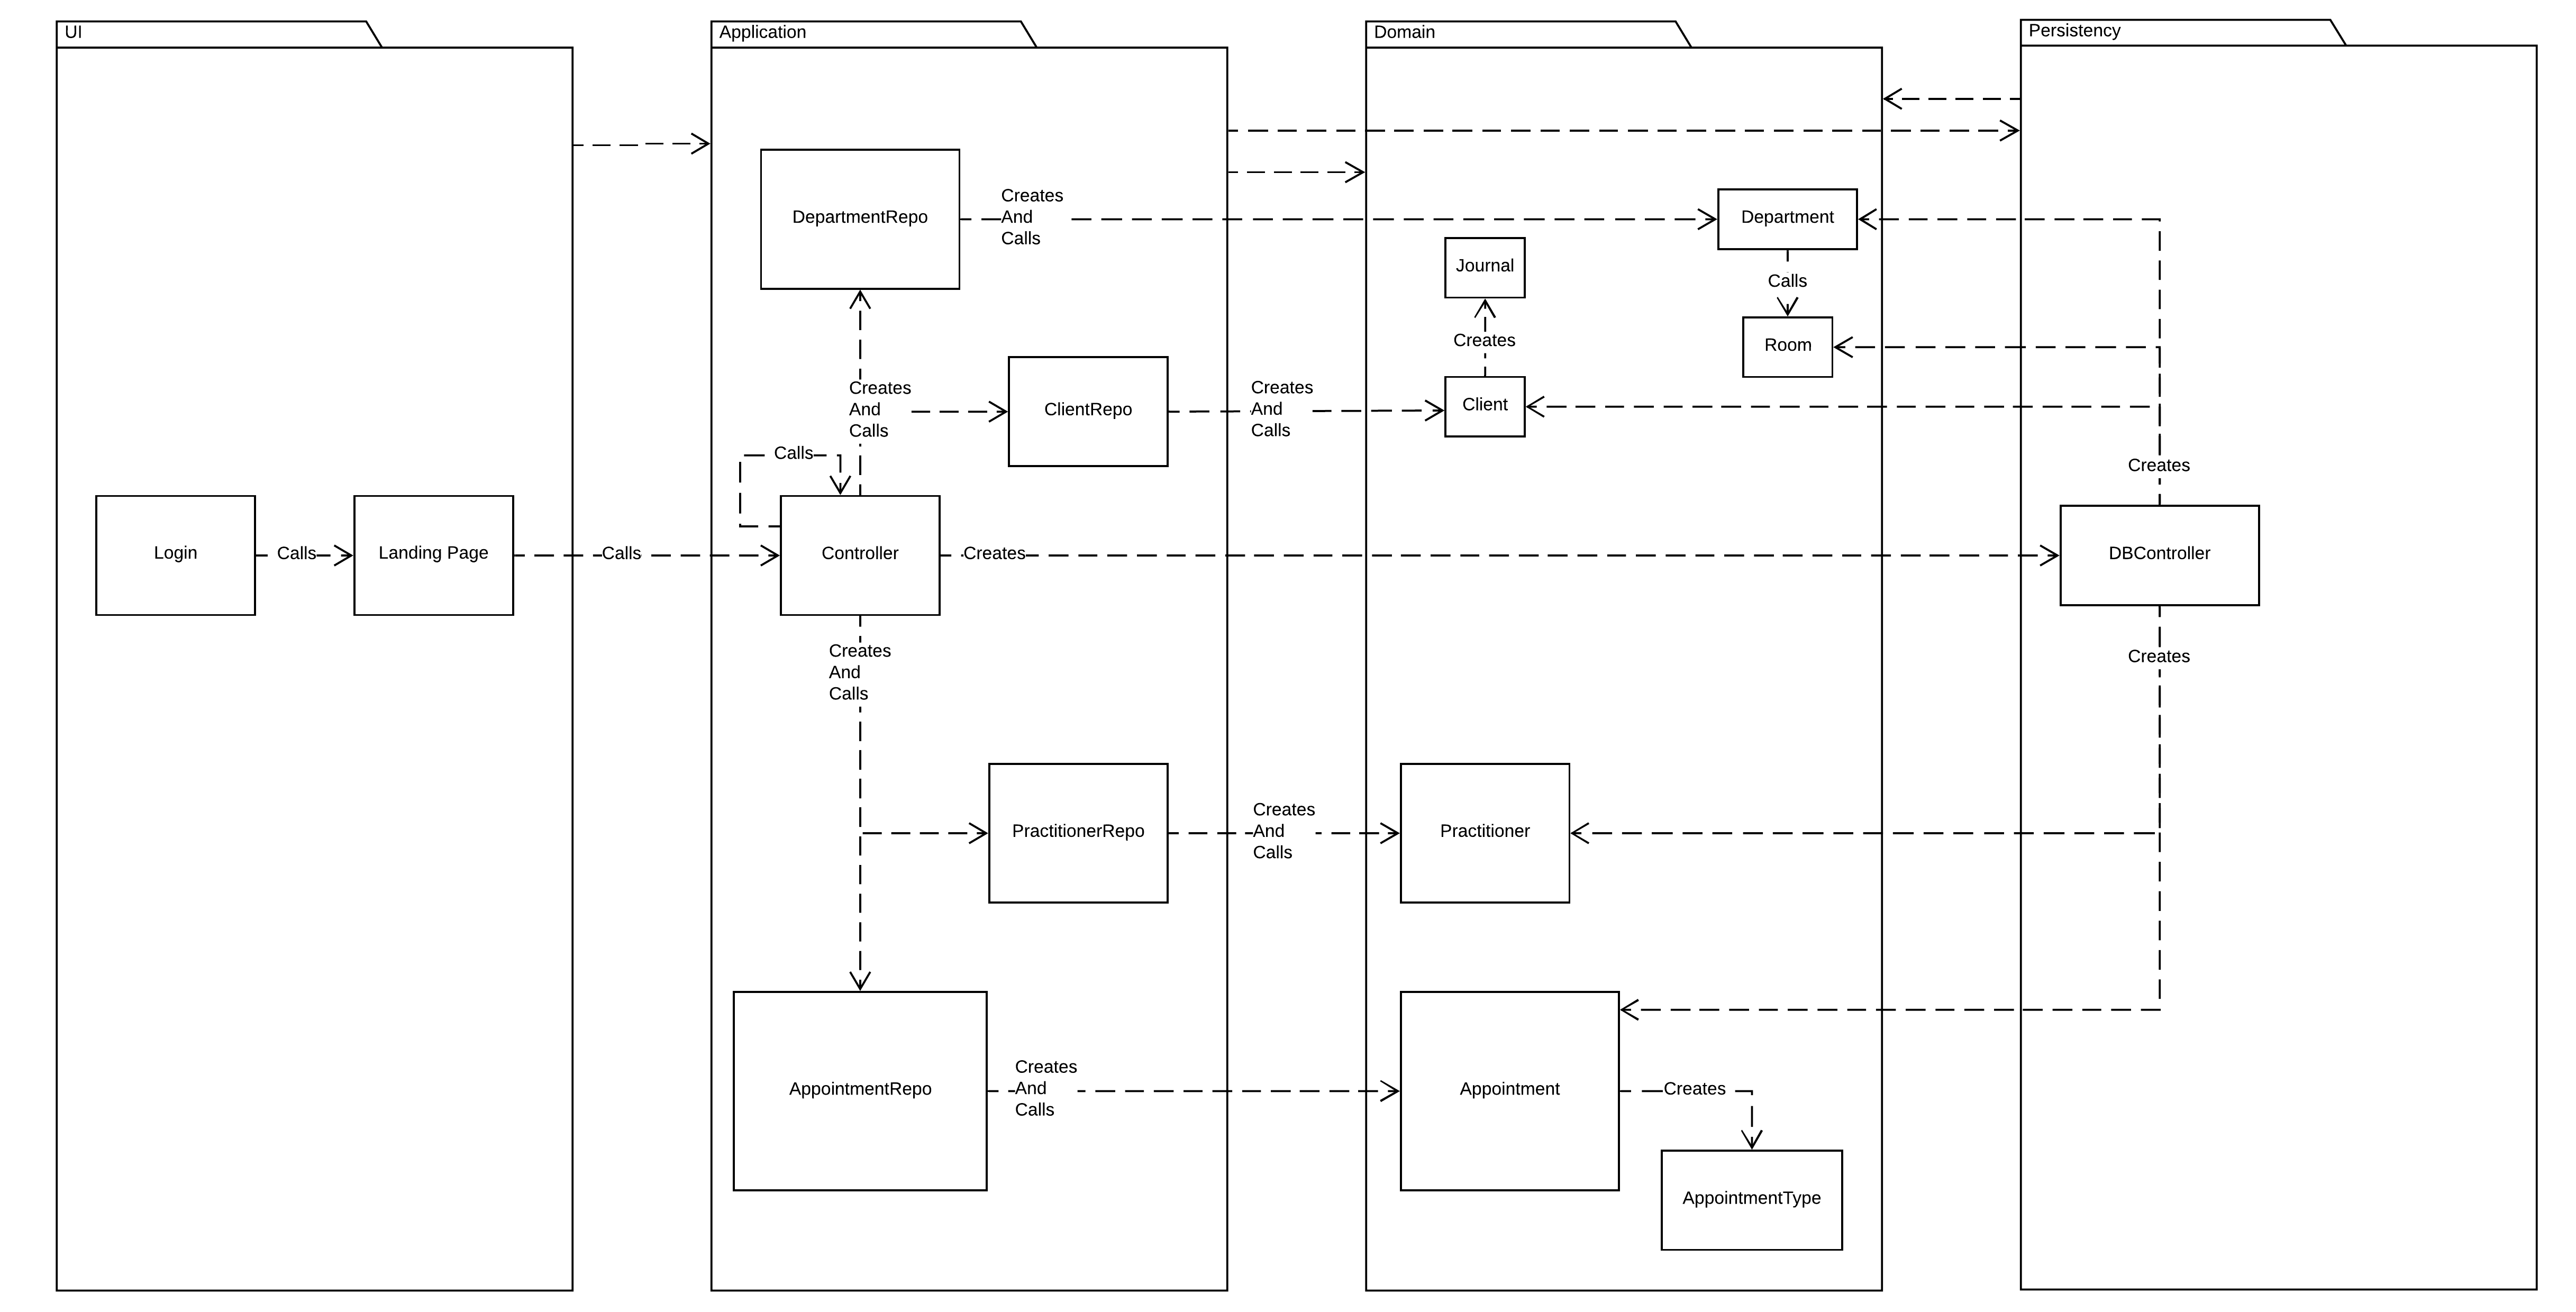
\includegraphics[width=\textwidth]{Pakkediagram.png}
    \label{fig:pakkediagram}
\end{sidewaysfigure}

\section{Modellering af Semplitos database}
\label{kabitel:ModelleringDB}
Vores løsning benytter sig af en database til at gemme data og sikre, at alle brugere af systemet kan tilgå dataene.

\subsection{Databasediagram(DBD)}
\label{DBD}

Vi har også opstillet et DBD for bedre at overskue opstillingen af databasen.
Opstillingen af DBD'et er gjort med udgangspunkt i vores domænemodel og DCD.
Ved at betragte domænemodellen og diskutere hvilke domæneklasser, det er nødvendigt at opbevare information om i vores database, har vi designet vores DBD, som kan ses på figur \ref{fig:DBD}.

Diagrammet i sig selv har været til stor hjælp - især ved normalisering af vores tabeller. 

\begin{figure}[H]
    \caption{Databasediagram for systemet}
    \centering
        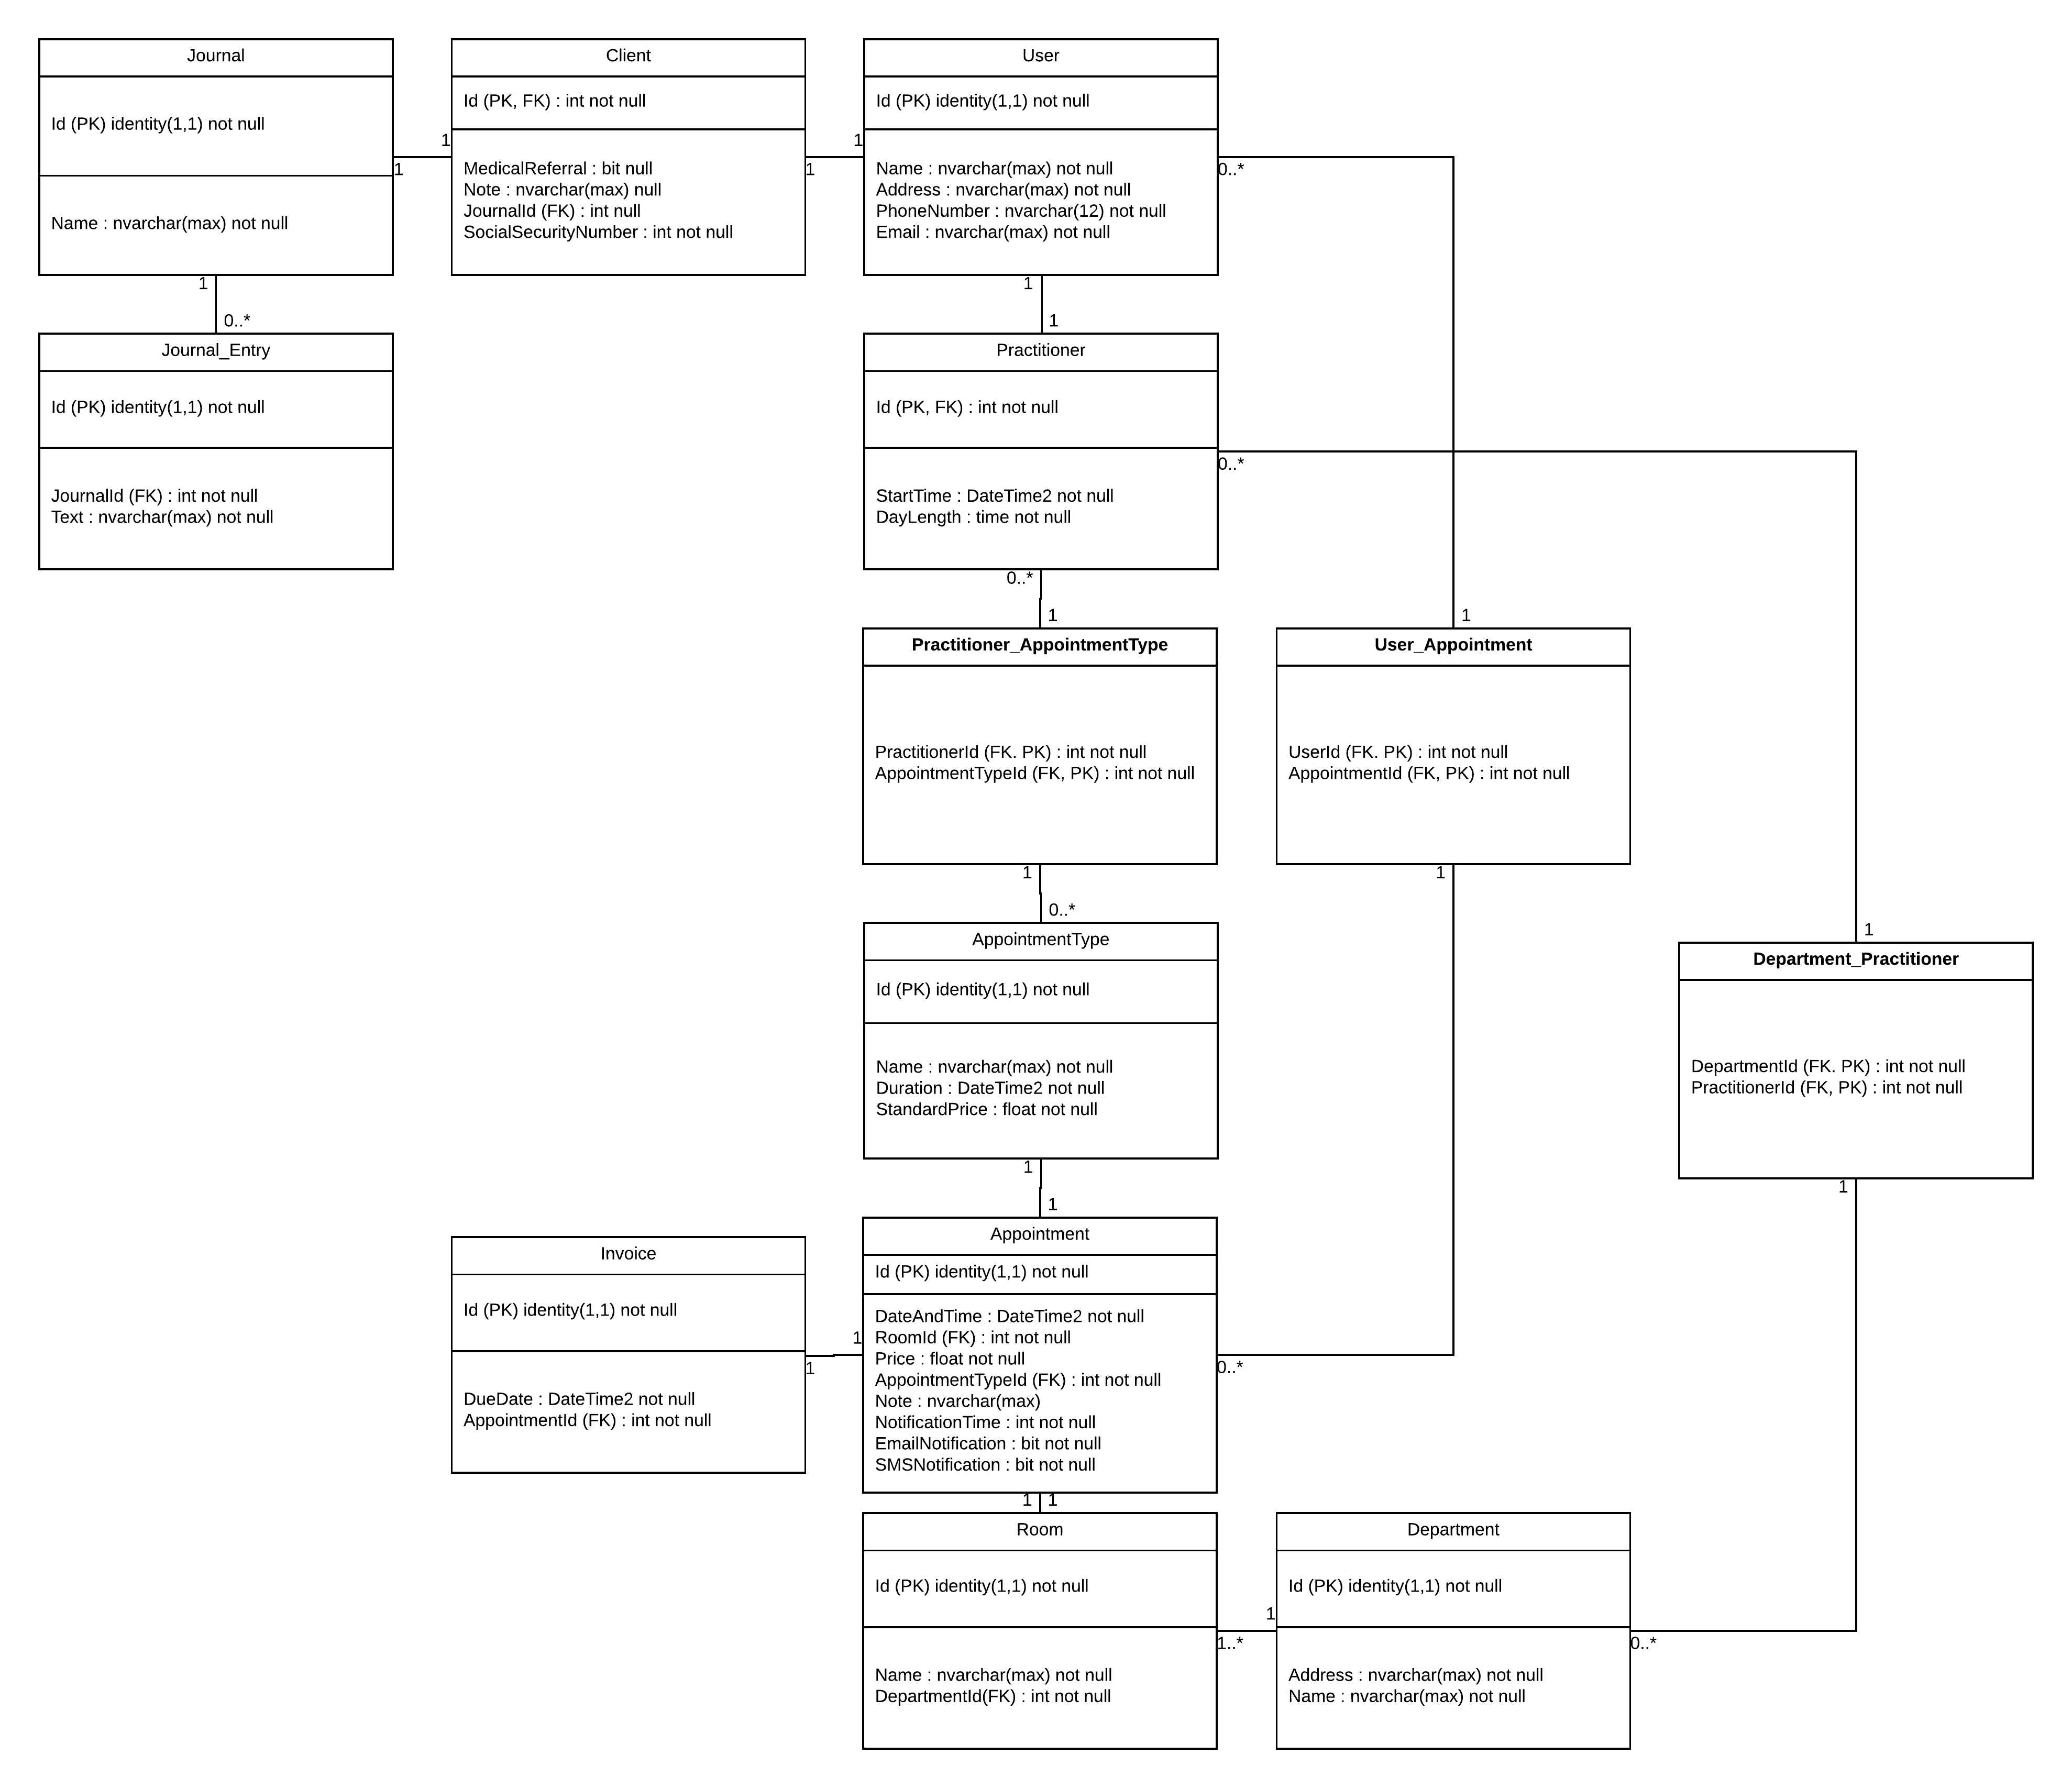
\includegraphics[width=\textwidth]{DBD.png}
    \label{fig:DBD}
\end{figure}

\subsubsection{Relationel database}

Vi har valgt at bruge en relationel database; hvor alt data er repræsenteret som tupler grupperet i relationer.
Den relationelle model blev først beskrevet af Edgar F. Codd i 1969.
Vi har valgt at bruge denne type af database, da vi har mange domæneklasser, der har forskellige sammenhænge, som det kan ses på figur \ref{system:domaene}.

Hvis vi blot havde vores database som en lang liste af datapunkter, ville det give problemer.
Man kan forestille sig, at PsykologNord ansætter en ny behandler, som endnu ikke har nogen aftaler.
Det ville betyde, at vi ville have en masse tomme værdier i resten af den række, hvor behandlerens informationer står.\cite{database}

I stedet deles den store tabel op i mindre tabeller, der indeholder referencer til hinanden.

\subsubsection{Normalisering af databasediagrammet}

For at læse teori om normalisering af databaser se bilag \ref{bilag:normalisering} på side \pageref{bilag:normalisering}. 

Måden vi har normaliseret vores database er ved først at identificere alle funktionelle afhængigheder, og så opstille tabeller, så alle determinanter er kandidatnøgler.
De er ikke alle primærnøgler, da vi har valgt at bruge substitutnøgler som primærnøgler.

Vores databasediagram kan ses på figur \ref{fig:DBD}.

\subsubsection{Views}

Et view er en virtuel tabel, hvis indhold defineres ud fra en forespørgsel.
Et view kan bruges som et filter til databasen, så man kan bestemme, hvordan hver enkelte bruger ser databasen.
Desuden kan det også bruges til at samle flere databaser og præsentere dem til brugeren som én database.

Vi bruger ikke på nuværende tidspunkt views i vores database, men det kunne have været fordelagtigt, at de stored procedures vi bruger til at hente informationer fra databasen hentede data fra views i stedet for at hente data direkte fra databasen.
Hvis vi ændrer databaseopbygningen nu, skal vi også ændre vores stored procedures og muligvis også vores kode i vores program, hvor, hvis vi brugte views, ville vi blot skulle ændre viewet, så det præsenterer dataene på samme måde som inden ændringen i databasen.

\subsubsection{Stored Procedures}
En stored procedure (SP) er gemt SQL forespørgsler, så det nemt kan køres igen, når det skal bruges.
Man kan bruge stored procedures til at bestemme, hvordan en bruger kan interagere med ens database ved at sætte rettighederne, så brugeren kun kan køre allerede eksisterende stored procedures.
Det er blevet lavet forskellige SP'er primært ud fra CRUD princippet, og en oversigt kan ses på figur \ref{StoredProcedures}.

\begin{figure}[h]
    \caption{Stored Procedures}
    \centering
        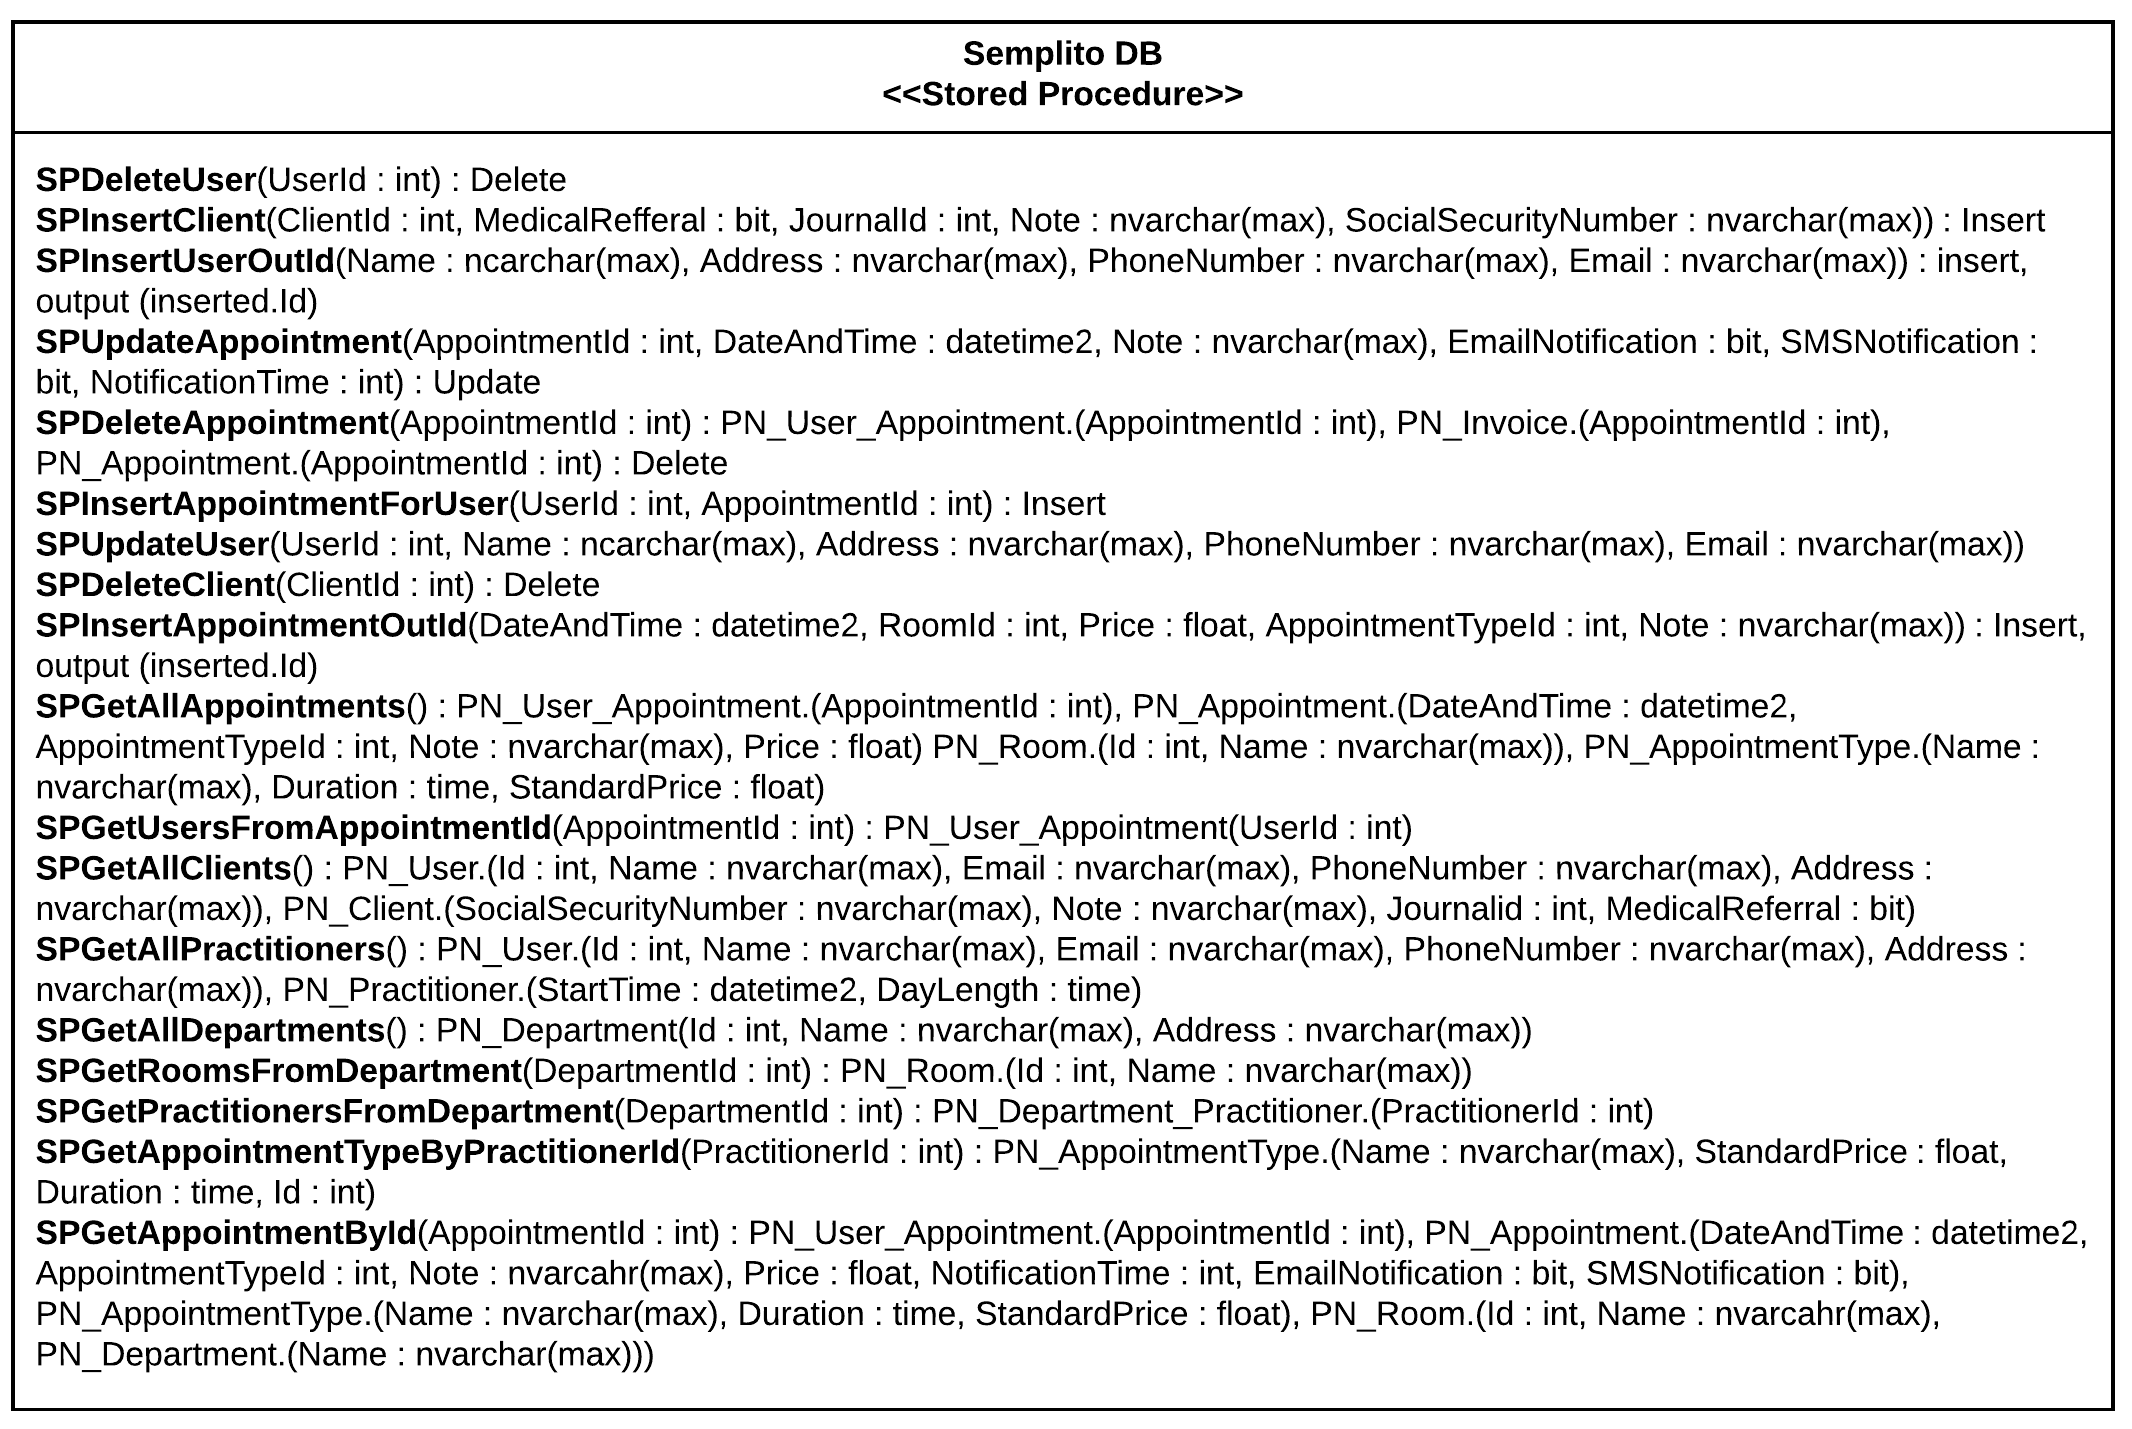
\includegraphics[width=\textwidth]{SP.png}
    \label{StoredProcedures}
\end{figure}

Vi har valgt at beskrive SP'en SPGetAllAppointments, se figur \ref{SPGetAllAppointments}, for at vise hvordan man kan bruge JOIN til at hente fra flere forskellige tabeller og få et enktelt table som output.

\begin{figure}[h]
    \caption{SPGetAllAppointments}
    \centering
        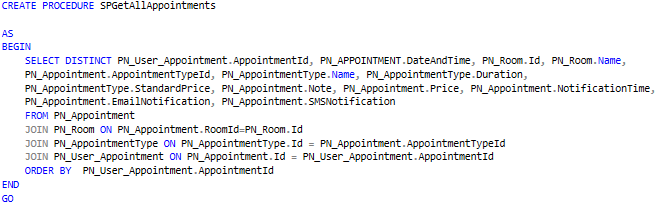
\includegraphics[width=\textwidth]{SPGetAllAppointments.png}
    \label{SPGetAllAppointments}
\end{figure}

Der er blevet brugt SELECT DISTINCT, som sørger for, at der ikke er nogle gentagelser af data i outputted.
Vi brugte det som et debugging værktøj, hvor det ikke er blevet fjernet, fordi vi gerne ville være sikre på, at der ikke var gentagelser.
Der er blevet brugt fire JOIN's i denne SP, keyworded JOIN i MSSQL er i sig selv et LEFT JOIN dvs. at den tager alt fra den første table og forener på det, de har tilfælles. Det gøres ved keyworded ON, hvor der efter bliver lavet en sammenligning på deres primary key og den modsatte tables foreign key.
Til sidst er der blevet brugt ORDER BY, som sørger for, at den kommer i den rækkefølge, som vi gerne vil have det i.
